\documentclass[11pt]{article}
\usepackage[margin=1in]{geometry}
\usepackage{amsmath,amssymb,amsthm}
\usepackage{graphicx,booktabs,array,float}
\usepackage[hidelinks]{hyperref}
\newtheorem{theorem}{Theorem}
\newtheorem{proposition}[theorem]{Proposition}
\newtheorem{lemma}[theorem]{Lemma}
\newtheorem{corollary}[theorem]{Corollary}
\theoremstyle{remark}
\newtheorem{remark}[theorem]{Remark}
\newcommand{\Tz}{T_0}
\newcommand{\To}{T_1}
\newcommand{\Tob}{\overline{T}_1}
\newcommand{\Tzb}{\overline{T}_0}
\newcommand{\sq}{\sqrt{3}}

\title{Two convex polygons with only non-periodic tilings:\\ a computer-assisted dissection of an aperiodic monotile}
\author{Andrew Bayly\thanks{Code, computations and a first draft of this text were developed with the assistance of Claude (Anthropic); the author is responsible for the content. \texttt{andrew.bayly@mac.com}}}
\date{Draft of 8 October 2026 --- not peer reviewed}

\begin{document}
\maketitle

\begin{abstract}
Smith, Myers, Kaplan and Goodman-Strauss found a continuous family $\mathrm{Tile}(a,b)$ of non-convex polygons, containing the ``hat'', each of which tiles the plane but never with a translational symmetry. We cut one member, $\mathrm{Tile}(299,240)$, into five convex pieces: one heptagon $\Tz$, three pentagons $\To$ and one mirror-image pentagon $\Tob$. Using exact arithmetic we enumerate, for each prototile, all ways it can be surrounded by tiles of the set, in the sense of a ``corona'', and prune those that cannot be extended. The surviving coronas show that in every tiling by $\Tz$, $\To$ and their reflections, with no matching rules and no edge-to-edge requirement, the tiles group uniquely into copies of $\mathrm{Tile}(299,240)$. Consequently every such tiling is the dissection of a tiling by the parent tile and has no translational symmetry. The argument is computer assisted and has not been reviewed independently; we describe the checks that were made (an independent second implementation, mutation tests, and a test against genuine tilings obtained from the hat substitution system), and the assumptions on which the result depends. Because no convex polygon is an aperiodic monotile (Rao, unrefereed), two prototiles is, conditionally, the smallest possible number for convex polygons.
\end{abstract}

\section{Introduction}

A \emph{tile set} is aperiodic if it admits tilings of the plane but none of them has a nonzero translation among its symmetries. For a long time all known aperiodic sets needed several tiles or decorations (matching rules). Smith, Myers, Kaplan and Goodman-Strauss \cite{SMKG24} found a single aperiodic tile, the ``hat'', and showed that it lies in a continuous family $\mathrm{Tile}(a,b)$ of aperiodic tiles whose tilings are combinatorially equivalent. All of these tiles are non-convex polygons. Rao \cite{Rao17} reports by computer search that the 15 known families of convex pentagons that tile the plane are complete, so that no convex polygon can be an aperiodic monotile; this is relied on in \cite{SMKG24}, although to our knowledge Rao's proof has not appeared in a refereed journal.

It is therefore natural to ask for aperiodic \emph{sets} of convex polygons, and for the smallest such set. Sugimoto \cite{Sug24} has proposed sets of three convex polygons, obtained by dissecting $\mathrm{Tile}(1,1)$, without matching rules and without reflections; aperiodicity is left unproven there. A further paper \cite{Sug26} considers pairs of \emph{concave} polygons derived from the hat and turtle and leaves open whether any of them is aperiodic.

\paragraph{Result.} We dissect $\mathrm{Tile}(299,240)$ into five convex pieces: three congruent pentagons $\To$, a fourth pentagon that is the mirror image $\Tob$ of the first, and a heptagon $\Tz$ (Figure~\ref{fig:tile}, Table~\ref{tab:data}). Let $\Sigma=\{\Tz,\Tzb,\To,\Tob\}$, where the bar denotes mirror image.

\begin{theorem}\label{thm:main}
Assume the computational facts of Proposition~\ref{prop:comp} below. Then every tiling of the plane by isometric copies (including reflections) of $\Tz$ and $\To$ is obtained by cutting each tile of a tiling of the plane by copies of $\mathrm{Tile}(299,240)$ in the standard way, and the correspondence is bijective and local. In particular no such tiling has a nonzero translational symmetry. Tilings by $\Tz$ and $\To$ exist.
\end{theorem}

No matching rules are used, and tiles need not meet edge to edge. The set $\{\Tz,\To\}$ with reflections allowed therefore has two prototiles. By the result cited above, two is the smallest number of prototiles for an aperiodic set of convex polygons, \emph{if} Rao's classification is correct.

\paragraph{What is and is not claimed.} The proof rests on a finite enumeration carried out by computer in exact arithmetic (Section~\ref{sec:method}); it also uses the theorem of \cite{SMKG24} as published. There has been no independent review; the author could not delegate the verification, so Section~\ref{sec:verif} describes in detail what was checked, and all code is public.\footnote{\url{https://github.com/andrewbayly/aperiodic_convex_polygons}} We prove the statement for the single parameter point $(299,240,208)$. Numerical experiments suggest that a two-parameter region of dissections behaves in the same way (Section~\ref{sec:family}), so there may be an infinite family of such aperiodic pairs; we have not attempted to prove this.

\begin{figure}[ht]
\centering
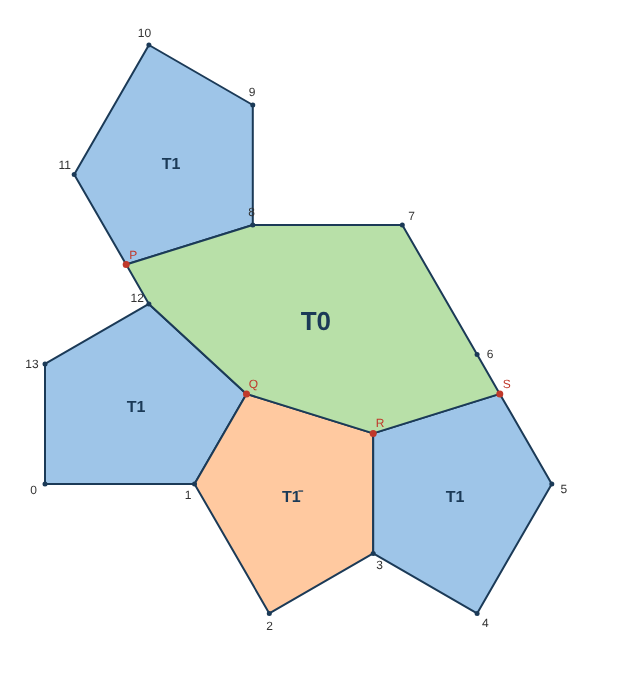
\includegraphics[width=0.62\textwidth]{figures/tile_Q.png}
\caption{The dissection of $\mathrm{Tile}(299,240)$. Vertices $0,\dots,13$ are those of the 14-gon; $P,Q,R,S$ are the cut points. The three blue pieces are copies of $\To$, the orange piece is $\Tob$, the green piece is $\Tz$.}\label{fig:tile}
\end{figure}

\section{The tile and its dissection}

Following \cite[Section 6]{SMKG24}, $\mathrm{Tile}(a,b)$ is the polygon with $14$ vertices $0,\dots,13$ (vertex $6$ is a straight $180^\circ$ vertex, so the polygon has 13 corners), interior angles
\[90^\circ,\,240^\circ,\,90^\circ,\,240^\circ,\,90^\circ,\,120^\circ,\,180^\circ,\,120^\circ,\,270^\circ,\,120^\circ,\,90^\circ,\,120^\circ,\,270^\circ,\,120^\circ\]
at vertices $0,\dots,13$, and sides $i\to i{+}1$ of length
\[a,\,a,\,b,\,b,\,a,\,a,\,a,\,a,\,b,\,b,\,a,\,a,\,b,\,b.\]
The hat is $\mathrm{Tile}(1,\sqrt3)$, and $\mathrm{Tile}(a,b)$ is aperiodic for every positive $b/a\neq1$ \cite{SMKG24}. We always allow reflections, as in \cite{SMKG24}, where the hat itself needs both reflected and unreflected copies.

\paragraph{The cuts.} Let $d>0$ be a parameter. Put $P$ on side $11\to12$ at distance $d$ from vertex $11$, and $Q$ on the bisector of the interior angle at vertex $1$ at distance $d$ from vertex $1$. Let $R$ be the reflection of vertex $12$ in the line $1Q$, and $S$ the reflection of $Q$ in the line $3R$. Cutting along the segments $8P$, $12Q$, $1Q$, $QR$, $R3$ and $RS$ divides the tile into five convex pieces:
\begin{align*}A&=[0,1,Q,12,13], & B&=[1,2,3,R,Q], & C&=[3,4,5,S,R],\\ D&=[8,9,10,11,P], & H&=[7,8,P,12,Q,R,S]\end{align*}
(with $S$ lying on side $5\to6$, so that vertex $6$ is absorbed into the side $S7$). With the same $d$ for both cuts, the pentagons $A$, $C$, $D$ are directly congruent and $B$ is their mirror image. We write $\To$ for $A$, $\Tob$ for $B$ and $\Tz$ for $H$. The dissection thus depends on three numbers $(a,b,d)$, i.e.\ on two shape parameters up to scale.

\paragraph{The chosen parameters.} We take $(a,b,d)=(299,240,208)$. The reason is arithmetic: the length $\ell=|Q12|$ equals $-275+312\sqrt3$ here, so that all vertex coordinates and all side lengths lie in $\mathbb Q(\sqrt3)$, and exact computation is possible in that field (for a generic parameter point $\ell$ generates a quartic extension). Table~\ref{tab:data} gives all coordinates, side lengths and angles.

\begin{table}[ht]
\centering\small
\renewcommand{\arraystretch}{1.15}
\begin{tabular}{@{}cll@{\qquad}cll@{}}
\toprule
vertex & $x$ & $y$ & vertex & $x$ & $y$\\
\midrule
$0$ & $0$ & $0$ & $9$ & $240\sq$ & $240+299\sq$\\
$1$ & $299$ & $0$ & $10$ & $120\sq$ & $360+299\sq$\\
$2$ & $\tfrac{897}{2}$ & $-\tfrac{299}{2}\sq$ & $11$ & $\tfrac{-299+240\sq}{2}$ & $\tfrac{720+299\sq}{2}$\\
$3$ & $\tfrac{897+240\sq}{2}$ & $\tfrac{240-299\sq}{2}$ & $12$ & $120\sq$ & $360$\\
$4$ & $\tfrac{897+480\sq}{2}$ & $-\tfrac{299}{2}\sq$ & $13$ & $0$ & $240$\\
$5$ & $598+240\sq$ & $0$ & $P$ & $\tfrac{-91+240\sq}{2}$ & $\tfrac{720+91\sq}{2}$\\
$6$ & $\tfrac{897+480\sq}{2}$ & $\tfrac{299}{2}\sq$ & $Q$ & $403$ & $104\sq$\\
$7$ & $299+240\sq$ & $299\sq$ & $R$ & $\tfrac{897+240\sq}{2}$ & $\tfrac{720-299\sq}{2}$\\
$8$ & $240\sq$ & $299\sq$ & $S$ & $494+240\sq$ & $104\sq$\\
\bottomrule
\end{tabular}

\medskip
{\footnotesize\begin{tabular}{@{}p{0.17\textwidth}p{0.27\textwidth}p{0.5\textwidth}@{}}
\toprule
prototile & sides (cyclic order) & interior angles (degrees, same order)\\
\midrule
$\To=A$, vertices $0,1,Q,12,13$ & $299,\,208,\,\ell,\,240,\,240$ & $90,\,120,\,102.666,\,107.334,\,120$\\[2pt]
$\Tz=H$, vertices $7,8,P,12,Q,R,S$ & $299,\,\ell,\,91,\,\ell,\,\ell,\,\ell,\,390$ & $120,\,162.666,\,77.334,\,162.666,\,154.669,\,145.331,\,77.334$\\
\bottomrule
\end{tabular}}
\caption{Exact coordinates of the vertices of $\mathrm{Tile}(299,240)$ (counterclockwise, vertex $0$ at the origin, side $0\to1$ along the $x$-axis) and of the cut points; and the data of the two prototiles, with $\ell=312\sqrt3-275\approx265.400$. Angles are rounded; the computation uses exact unit vectors.}\label{tab:data}
\end{table}

\section{Method}\label{sec:method}

\subsection{Coronas}

Let $X$ be a tiling by $\Sigma$ and $c$ a tile of $X$. The \emph{corona} $C(c;X)$ is the smallest set of tiles of $X$ containing $c$ and containing every tile that has a corner at a point $p\in\partial c$ which is a corner of a tile already in the set. Tiles that touch $c$ only along an edge passing through such points are not necessarily included (this is deliberate; see ``partial tiles'' below). At every point of $\partial c$ that is a corner of a tile of $C(c;X)$, the plane is covered by the tiles of $X$ around it, but some of them (those with the point in the interior of a side) may not belong to $C(c;X)$.

\paragraph{Enumeration.} For a prototile $c$ in a fixed position we enumerate all candidate coronas by gap filling. A state is a finite set of tiles with disjoint interiors, together with a set of \emph{partial tiles} (below). At each point $v\in\partial c$ that is a corner of a tile of the state, the tiles around $v$ occupy a union of angular wedges, and the state is complete at $v$ if these wedges, together with the partial tiles at $v$, cover the full angle $2\pi$. If a vertex has an uncovered angular gap, consider the first ray of the gap (in counterclockwise order). In any tiling the tile of $X$ lying just beyond this ray either has a corner at $v$, with one of its sides along the ray (we try every corner of every element of $\Sigma$ whose angle does not exceed the gap), or has $v$ in the interior of a side (``partial tile''; only possible if the gap is at least $\pi$). Partial tiles are not placed; they are recorded as a straight wedge of $\pi$ at $v$ whose position along the side is left free. If later a placed tile realises exactly that straight wedge at $v$, the record is removed (it stood for that tile). We always treat next the gap of smallest angle. A branch is abandoned when two tiles overlap, when wedges at a vertex overlap, or when no option remains for the chosen gap. The result is a finite list of states with no remaining gap, the \emph{first coronas} of $c$.

\begin{lemma}[Completeness of the enumeration]\label{lem:complete}
For every tiling $X$ by $\Sigma$ and every tile $c$ of $X$, after moving $c$ to its reference position the corona $C(c;X)$ is among the states enumerated for $c$.
\end{lemma}
\begin{proof}[Proof (sketch)]
Follow $X$ along the search: at each step the tile of $X$ just beyond the first ray of the chosen gap is one of the options tried (a corner of some prototile at $v$, with a side on the ray, or a partial tile); choose that one. All tiles placed are tiles of $X$ in $C(c;X)$, because each is placed at a point of $\partial c$ which is a corner of a tile already placed. No branch is abandoned (disjointness and angle sums hold in $X$). When no gap remains the state consists of exactly the tiles of $C(c;X)$: a tile of $C(c;X)$ has a corner at a point of $\partial c$ that is a corner of an earlier tile, and would have been placed when that point's gap was filled. \qedhere
\end{proof}

\subsection{Pruning}

A first corona $C$ of $c$ is \emph{refuted} if some tile $t\in C$ cannot itself be surrounded: starting from the state $C$ (including its partial tiles) we run the same enumeration for the vertices on $\partial t$ and find no complete state (within a node budget; if the budget is exhausted the corona is conservatively kept). The remaining coronas are the \emph{survivors}.

\begin{lemma}[Survivors contain all true coronas]\label{lem:sound}
For every tiling $X$ by $\Sigma$ and every tile $c$ of $X$, $C(c;X)$ is a survivor.
\end{lemma}
\begin{proof}
By Lemma~\ref{lem:complete} it is a first corona. For $t\in C(c;X)$ the same argument applied to $t$ (the search follows $X$, starting from the state $C(c;X)$ and using that all its tiles are in $X$) produces a complete state, so $C(c;X)$ is not refuted. \qedhere
\end{proof}

\subsection{Exact arithmetic and implementation}

All vertex coordinates of all tiles lie in $\mathbb Q(\sqrt3)$. Directions of sides are represented by exact unit vectors; angles are compared and added by exact complex arithmetic in the field generated by the unit vectors; tests for overlap of two convex polygons use exact separating-axis tests. Floating point is used only as a prefilter and its answer is accepted only when it is clear by a margin of $10^{-6}$; otherwise the exact test decides. The primary implementation (JavaScript with arbitrary-precision integers) and a second, independent implementation (Python with rational numbers in $\mathbb Q(\sqrt3)$, different data structures, different search order) are in the repository.

\section{Results}

\begin{proposition}[Computation]\label{prop:comp}
Let $a=299$, $b=240$, $d=208$.
\begin{enumerate}
\item[(a)] $\Tz$ has $18$ first coronas, of which $2$ survive. Each survivor contains, besides $\Tz$, four tiles lying exactly in the positions of the pieces $A,B,C,D$; that is, $\Tz$ together with these tiles is a copy of $\mathrm{Tile}(299,240)$ cut as above.
\item[(b)] $\To$ has $368$ first coronas, of which $25$ survive. Each survivor contains a tile $\Tz$ or $\Tzb$ situated, relative to $\To$, exactly as the piece $H$ is situated relative to one of the pieces $A$, $C$, $D$ of an unreflected copy of the parent tile, or relative to $B$ in a reflected copy; and it contains such a tile for exactly one of these four roles. The 25 survivors split by role as $5$ ($A$), $11$ ($C$), $4$ ($D$), $5$ ($B$, reflected).
\item[(c)] The results for $\Tzb$ and $\Tob$ are the mirror images of (a), (b).
\end{enumerate}
\end{proposition}

\begin{figure}[ht]
\centering
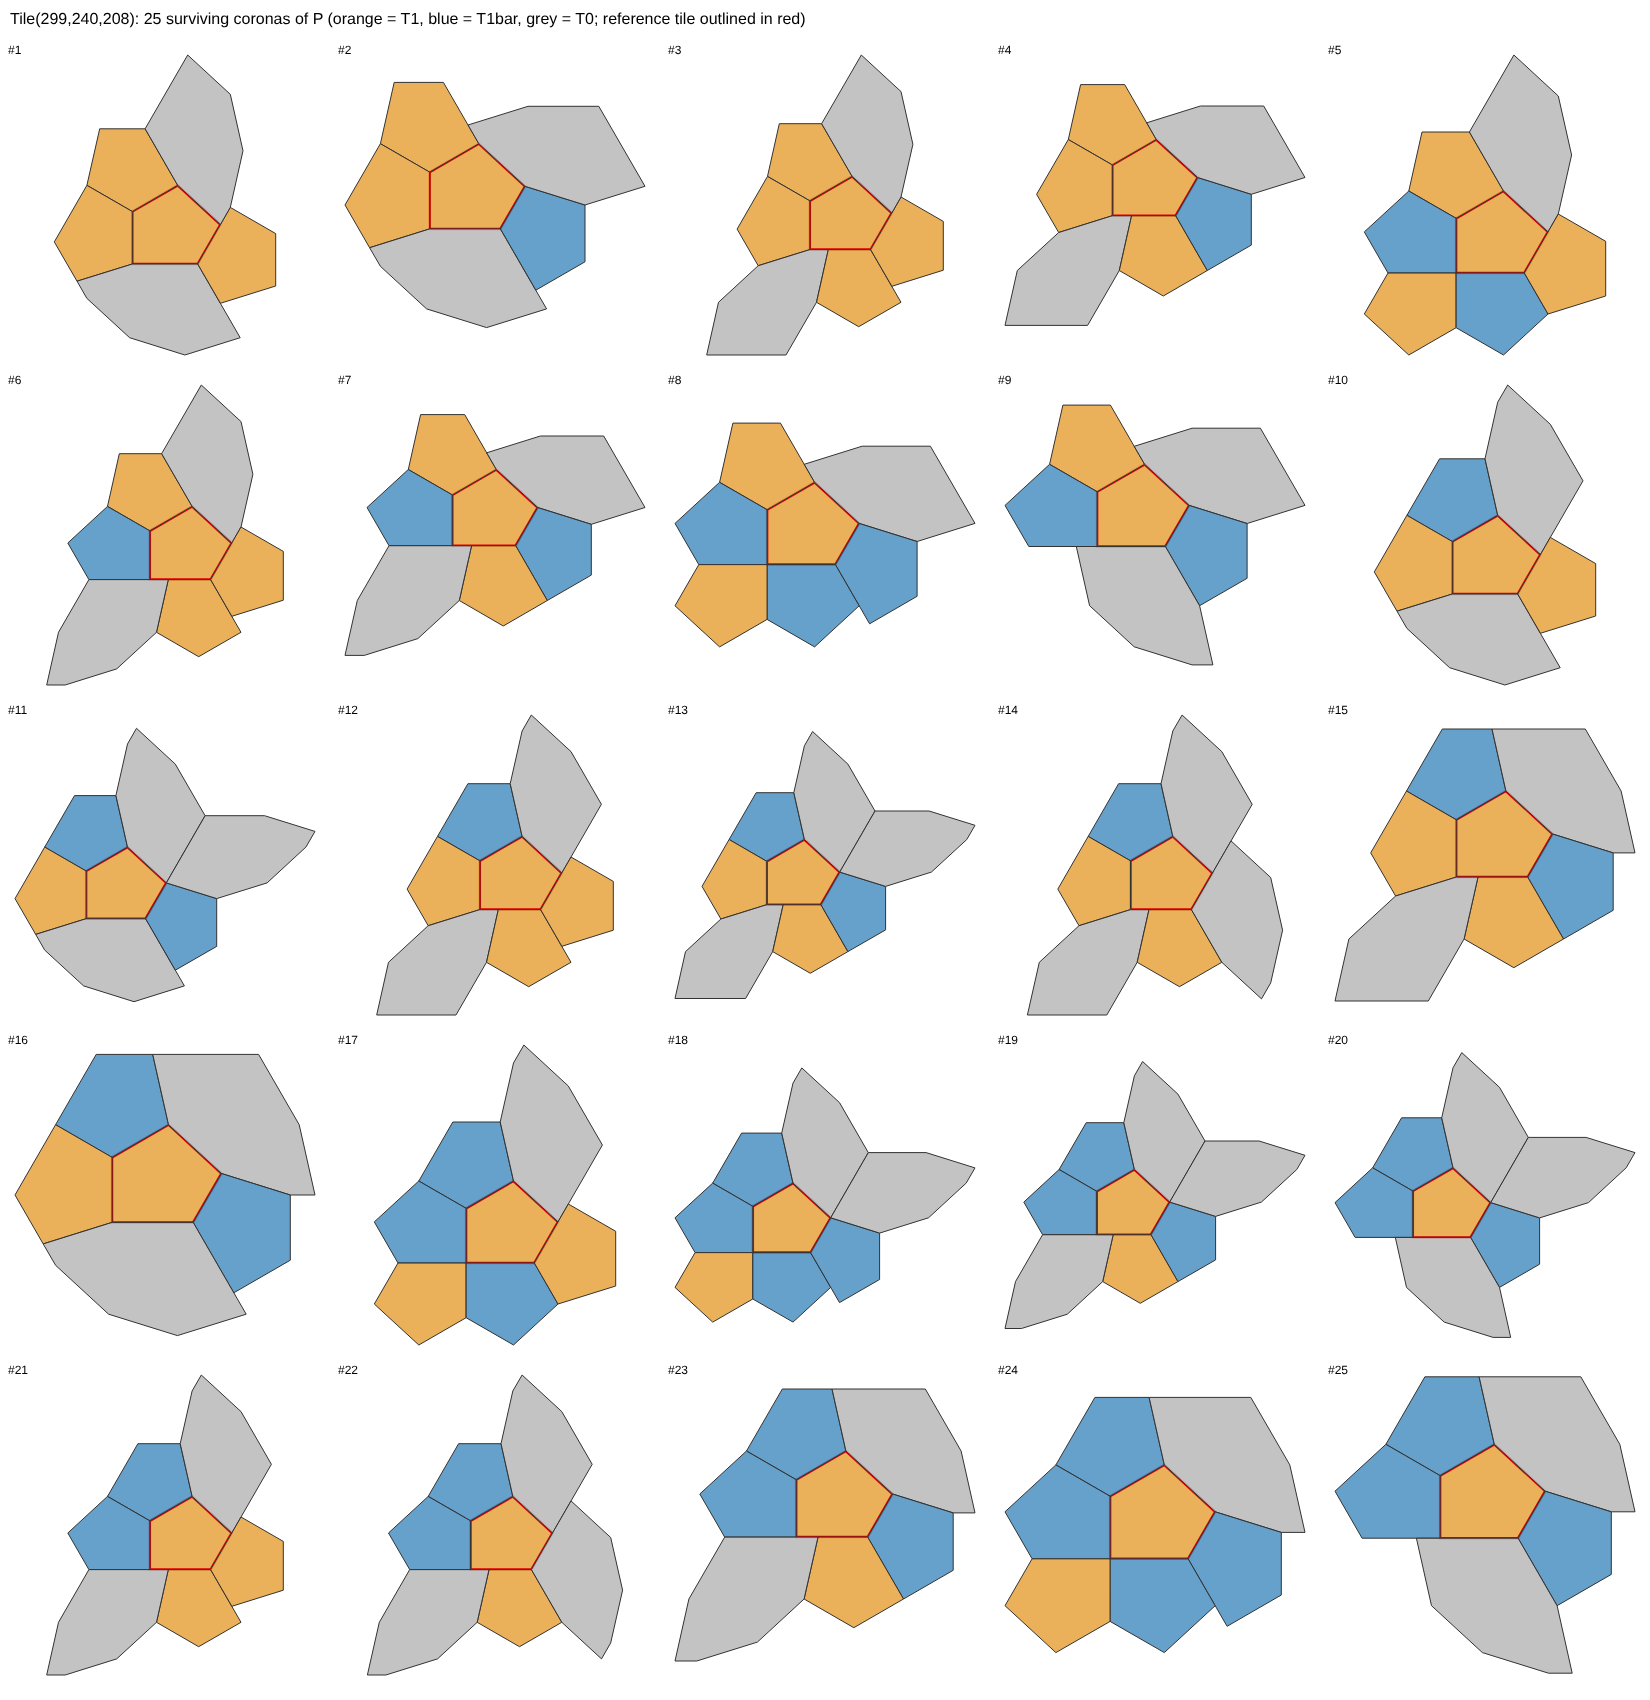
\includegraphics[width=\textwidth]{figures/survivors_T1.png}
\caption{The 25 surviving coronas of $\To$ (reference tile outlined in red; orange: $\To$, blue: $\Tob$, grey: $\Tz$).}\label{fig:surv1}
\end{figure}
\begin{figure}[ht]
\centering
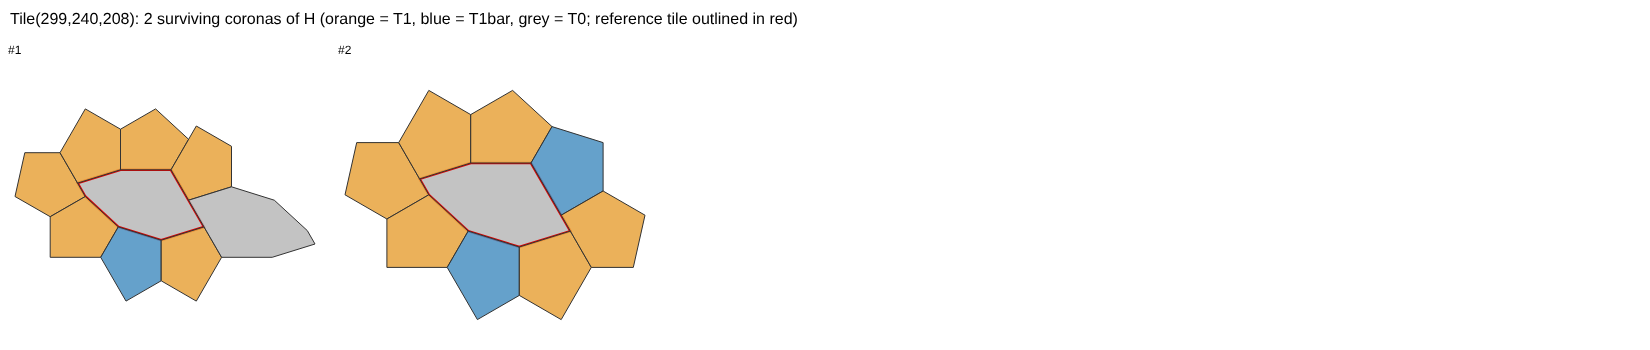
\includegraphics[width=\textwidth]{figures/survivors_T0.png}
\caption{The 2 surviving coronas of $\Tz$. Each contains the other four pieces of a parent tile.}\label{fig:surv0}
\end{figure}

\begin{proof}[Proof of Theorem~\ref{thm:main}, given Proposition~\ref{prop:comp}]
Let $X$ be a tiling by $\Sigma$. For a tile $h$ congruent to $\Tz$ or $\Tzb$, Lemma~\ref{lem:sound} and Proposition~\ref{prop:comp}(a),(c) show that $h$ lies in a unique copy $K(h)$ of the parent tile all of whose five pieces are tiles of $X$.

Now let $t$ be a tile congruent to $\To$ or $\Tob$. By Lemma~\ref{lem:sound} and Proposition~\ref{prop:comp}(b),(c) the corona of $t$ contains a tile $h$ (a copy of $\Tz$ or $\Tzb$) situated relative to $t$ as $H$ is relative to the piece playing a role $\rho$, for exactly one $\rho$. The cluster $K(h)$ contains a tile in the position of that piece; this tile and $t$ occupy the same polygon, so they are the same tile and $t\in K(h)$.

The clusters are disjoint: suppose a tile $t$ lies in two clusters $K(h)$ and $K(h')$. Each of $A,B,C,D$ shares a segment of its boundary with $H$, so $h$ and $h'$ both belong to the corona of $t$, each situated relative to $t$ as $H$ relative to the piece $t$ plays in the respective cluster. Since $t$ witnesses exactly one role, these two roles coincide, hence $h=h'$.

So the tiles of $X$ are partitioned into clusters $K(h)$, each a copy of the parent tile, with disjoint interiors and covering the plane: they form a tiling $Y$ by $\mathrm{Tile}(299,240)$. The cluster of a tile depends only on its corona; hence $X\mapsto Y$ is local, and it commutes with all isometries. Cutting the tiles of $Y$ gives $X$ back, and conversely cutting the tiles of any tiling $Y'$ by $\mathrm{Tile}(299,240)$ gives a tiling $X'$ by $\Sigma$ with $X'\mapsto Y'$ (the cluster found for a piece is the parent tile, because the parent is a cluster in which the piece plays a role, and the role is unique). A translation that is a symmetry of $X$ is therefore a symmetry of $Y$. By \cite[Theorem~1.1 and Section~6]{SMKG24}, $\mathrm{Tile}(299,240)$ admits no tiling with a translational symmetry. Hence $X$ has none. Tilings exist: $\mathrm{Tile}(299,240)$ tiles the plane (it is combinatorially equivalent to the hat \cite[Theorem 6.1]{SMKG24}); cut one. \qedhere
\end{proof}

\begin{figure}[ht]
\centering
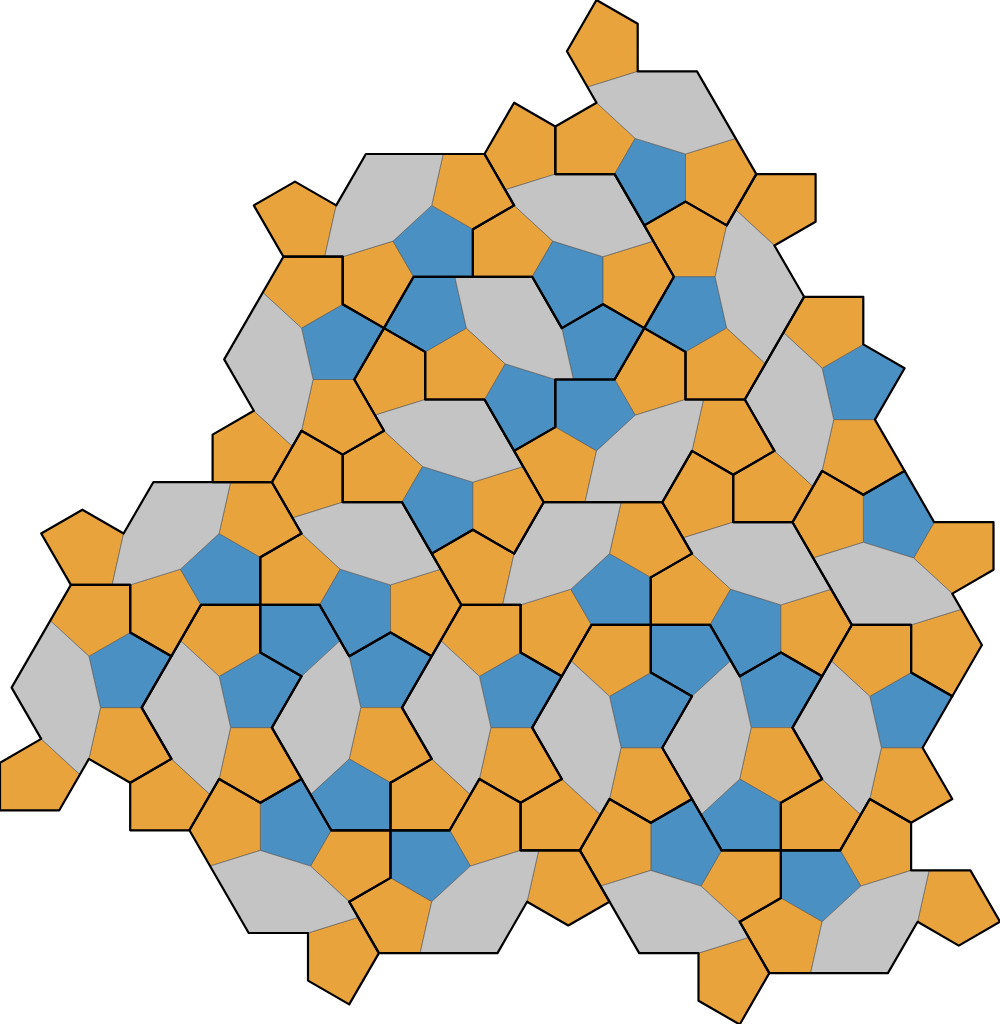
\includegraphics[width=0.85\textwidth]{figures/patch.png}
\caption{A patch of a tiling by $\Sigma$, obtained from a patch of the hat substitution tiling (Section~\ref{sec:verif}) realised as $\mathrm{Tile}(299,240)$ and cut. Parent tiles are outlined in black.}\label{fig:patch}
\end{figure}

\begin{corollary}[conditional minimality]
If no convex polygon is an aperiodic monotile \cite{Rao17}, then no aperiodic set of convex polygons has fewer than two elements, so $\{\Tz,\To\}$ (with reflections) has the least possible number of prototiles.
\end{corollary}

\section{Verification}\label{sec:verif}

Because the argument is computer assisted and was produced by a single author, we describe what was done to protect against errors. All of it can be repeated with the script \texttt{verify.sh} of the repository.

\paragraph{Exact arithmetic.} No geometric decision relies on floating point alone (Section~\ref{sec:method}). The number of such decisions that were not settled by the float prefilter is recorded by the programs.

\paragraph{Independent implementation.} A second program, written without sharing code or data structures with the first, produces precisely the same sets of first coronas and survivors for $\Tz$ and $\To$ (18, 2 and 368, 25; identical as sets). It also agrees with the first on every run that completes within a node cap, in a test of 30 further, artificially generated tile sets. Comparing the two programs found one real error during development: partial tiles were never removed once the tile they stood for was placed, so a valid branch looked over-covered and was discarded. The corrected programs agree; the error changed the counts (for example $20$ instead of $25$ survivors for $\To$).

\paragraph{Mutation tests.} We introduced seven deliberate faults into the engine, one at a time: no partial tiles; the original error described above; omitting one corner type; requiring corners strictly smaller than a gap; partial tiles only for gaps much larger than $\pi$; disabling the polygon-overlap test; and not detecting overlapping wedges. The first five remove legal placements and each changes the results visibly (for $\To$ the counts of first coronas and survivors become $232/20$, $232/20$, $49/1$, $0/0$, $232/20$ instead of $368/25$). The last two do not remove placements: the overlap test is redundant at these parameters (no change), and ignoring overlapping wedges adds spurious survivors ($452/31$).

\paragraph{Genuine tilings.} Lemma~\ref{lem:sound} is the step where an error would be most damaging, since a corona wrongly discarded would remove a case from the proof. We therefore tested it against real tilings. A patch of the hat substitution tiling was generated with the code of Kaplan \cite{hatviz} (7921 tiles). Each hat was matched exactly to $\mathrm{Tile}(1,\sqrt3)$; vertices were graded by the numbers of sides of length $a$ and $b$ along edge paths, translations were propagated over shared vertices, and the patch was re-realised with $(a,b)=(299,240)$. The grading is consistent at every shared vertex, which is the fact underlying \cite[Theorem 6.1]{SMKG24}. Cutting gives a tiling patch by $\Sigma$ with 39\,605 pieces (Figure~\ref{fig:patch}). For the 30\,335 pieces whose neighbourhood of radius about the size of a parent tile lies inside the patch we formed the true corona and looked it up: all 30\,335 are among the survivors, none was discarded. These coronas realise 16 of the 25 survivors of $\To$ (and 8 of the 25 survivors of $\Tob$; 20 of 25 after identifying mirror images) and both survivors of $\Tz$. Survivors that never occur are permitted by Lemma~\ref{lem:sound} and do not affect the argument, because each survivor displays a role. The same test, run against the engine with the faults above, fails for every fault that removes legal placements, including the original error (15 of 245 true coronas lost in a small patch), and does not detect the two faults that only enlarge the survivor set.

\paragraph{Limits of the checks.} The test uses patches of the substitution tiling only; \cite{SMKG24} note that tilings with infinite fault lines are not known to be excluded, so coronas occurring only along such lines are not sampled (the theorem itself does not depend on this, since it quantifies over all tilings, but its computational basis, Lemma~\ref{lem:complete}, is a statement about all tilings and is not tested there). The agreement of two programs by the same author does not exclude a common misreading of the definitions. Node budgets in the pruning were never exhausted at the chosen parameters (no corona was kept for that reason).

\section{Other parameter values}\label{sec:family}

For $b=1$ and a grid of values of $a$ and $d$ we constructed the dissection numerically and ran the same enumeration in floating point (Figure~\ref{fig:param}). At each of 226 of the 440 grid points the five pieces are convex and the enumeration gives the same pattern as above (2 survivors for $\Tz$ and 25 for $\To$ with role counts $5,11,4,5$); at 212 points a piece is non-convex and at 2 points the pieces are inconsistent. The valid points form an L-shaped region and $(299,240,208)$ lies well inside it. This is evidence only: the floating-point runs are not proofs, and the region $a/b>2$, $d/b>0.5$ was not scanned. We have not tried to prove the statement for the whole region.

\begin{figure}[ht]
\centering
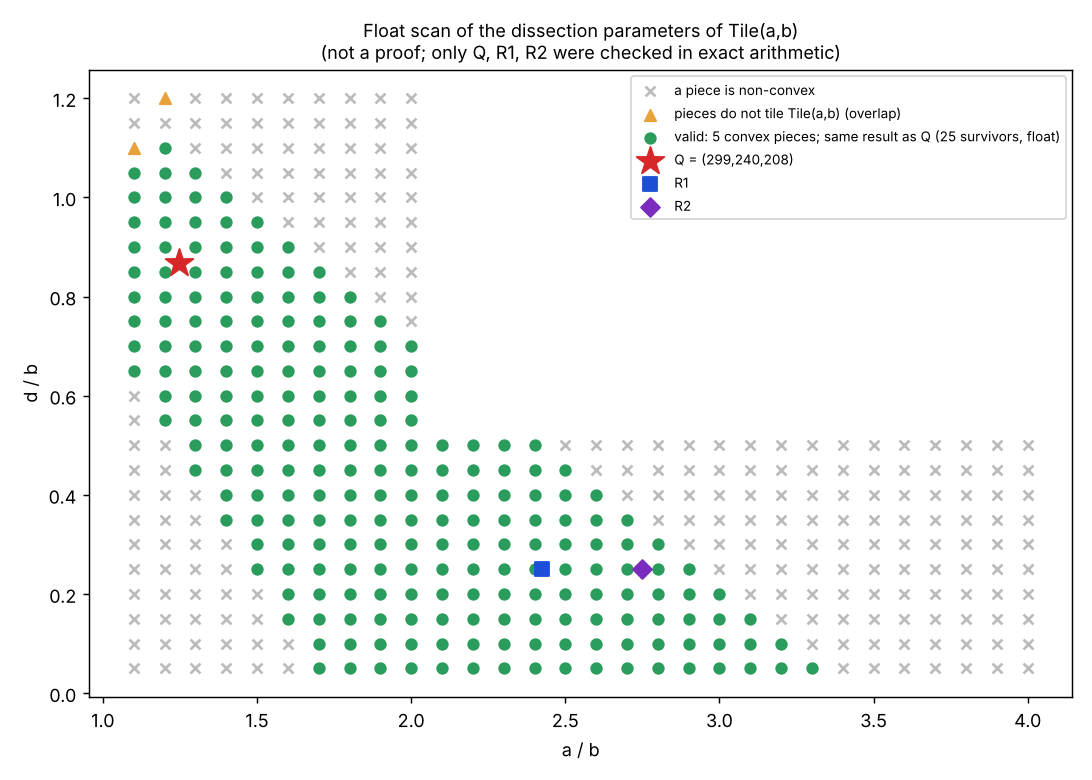
\includegraphics[width=0.8\textwidth]{figures/parameter_region.png}
\caption{Floating-point scan of the dissection parameters ($b=1$). Green points reproduce the pattern proved above for $(299,240,208)$ (red star).}\label{fig:param}
\end{figure}

\section{Discussion and open questions}

\begin{itemize}
\item \textbf{Dependence on external results.} (i) The aperiodicity of $\mathrm{Tile}(a,b)$ \cite{SMKG24}, published; we use only the statement for $b/a=240/299$ (Theorem 6.1 transfers the hat's absence of periodic tilings to this case). (ii) For the minimality statement, Rao's classification \cite{Rao17}, which we do not re-prove; the preprint reports a computer search. Hales reported (blog post, 2017) verifying part of it. A refereed statement would be welcome.
\item \textbf{Computer assistance.} The enumeration is small (368 and 18 first coronas) and is reproducible in minutes (the independent implementation takes about 17 minutes), but a human-checkable proof of Proposition~\ref{prop:comp} would be preferable.
\item \textbf{Open questions.} Is the pattern valid on a whole region of parameters, and can it be proved uniformly? Are there aperiodic sets of two convex polygons that do not arise as dissections of an aperiodic monotile? Can the use of reflections be avoided, as for the chiral monotile of \cite{SMKG23}?
\end{itemize}

\begin{thebibliography}{99}
\bibitem{SMKG24} D.~Smith, J.~S.~Myers, C.~S.~Kaplan, C.~Goodman-Strauss, \emph{An aperiodic monotile}, Combinatorial Theory \textbf{4}(1) (2024), \#6; arXiv:2303.10798.
\bibitem{SMKG23} D.~Smith, J.~S.~Myers, C.~S.~Kaplan, C.~Goodman-Strauss, \emph{A chiral aperiodic monotile}, arXiv:2305.17743.
\bibitem{Rao17} M.~Rao, \emph{Exhaustive search of convex pentagons which tile the plane}, arXiv:1708.00274 (2017).
\bibitem{Sug24} T.~Sugimoto, \emph{Aperiodic sets of three types of convex polygons}, arXiv:2404.00534.
\bibitem{Sug26} T.~Sugimoto, \emph{Tile sets consisting of two types of concave polygons derived from periodic tilings corresponding to non-periodic tilings with hat and turtle tiles}, arXiv:2609.09603 (2026).
\bibitem{hatviz} C.~S.~Kaplan, \emph{hatviz}, \url{https://github.com/isohedral/hatviz} (BSD 3-clause).
\end{thebibliography}

\end{document}
